\documentclass{article}
\usepackage{amsmath}
\usepackage{amssymb}
\usepackage{amsthm}
\usepackage{listings}
\usepackage{xcolor}
\usepackage{graphicx}

\title{Exam Solutions}
\author{}
\date{}

\begin{document}

\lstset{
  basicstyle=\ttfamily\footnotesize,
  keywordstyle=\color{blue},
  commentstyle=\color{gray},
  stringstyle=\color{red},
  breaklines=true,
  frame=single,
  numbers=left,
  numberstyle=\tiny,
  language=Python
}

\maketitle

\section*{Part 1}
Consider the advection diffusion equation given as
\begin{equation}
    \frac{\partial u(x, t)}{\partial t} + U_0(x) \frac{\partial u(x, t)}{\partial x} = \nu \frac{\partial^2 u(x, t)}{\partial x^2},
\end{equation}
where $U_0(x)$ is periodic and bounded and $\nu$ is assumed to be constant. Also $u(x, t)$ is assumed to be smooth and periodic as is the initial condition.

\subsection*{(a)}
State sufficient conditions on $U_0(x)$ and $\nu$ that ensures Eq. 1 to be well-posed.

\textbf{Solution:}
For the advection-diffusion equation to be well-posed, we need the following conditions:
\begin{enumerate}
    \item $\nu > 0$: This ensures that the diffusion term provides dissipation and prevents the solution from growing unboundedly.
    \item $U_0(x)$ should be Lipschitz continuous: This ensures that the advection term doesn't cause any singularities in the solution.
    \item The initial condition $u(x,0)$ should be in $L^2$ space: This ensures that the initial energy is finite.
\end{enumerate}
These conditions guarantee the existence, uniqueness, and continuous dependence of the solution on the initial data.

\subsection*{(b)}
Assume that Eq. 1 is approximated using Fourier Collocation method. Is the approximation consistent and what is the expected convergence rate when increasing $N$, the number of modes used in the approximation.

\textbf{Solution:}
The Fourier Collocation method for this equation is indeed consistent. The consistency can be shown by:
\begin{enumerate}
    \item The spatial derivatives are approximated using the discrete Fourier transform
    \item For smooth periodic functions, the Fourier approximation converges to the exact solution
\end{enumerate}

The convergence rate is spectral (exponential) in $N$ for smooth solutions. Specifically:
\begin{itemize}
    \item If $u(x,t)$ is infinitely differentiable, the error decreases faster than any power of $1/N$
    \item For solutions with finite regularity, the convergence rate is $O(N^{-k})$ where $k$ is the order of differentiability
\end{itemize}

\subsection*{(c)}
Assume now that $U_0(x)$ is constant and Eq. 1 is approximated using a Fourier Collocation method with odd number of modes. Prove that the semi-discrete approximation, i.e. continuous time and approximated space, is stable.

\textbf{Solution:}
Let's prove the stability of the semi-discrete approximation:

1. For constant $U_0$, the semi-discrete system can be written as:
\begin{equation}
    \frac{d\hat{u}_k}{dt} = (-ikU_0 - \nu k^2)\hat{u}_k
\end{equation}
where $\hat{u}_k$ are the Fourier coefficients.

2. The solution of this ODE is:
\begin{equation}
    \hat{u}_k(t) = \hat{u}_k(0)e^{(-ikU_0 - \nu k^2)t}
\end{equation}

3. For stability, we need to show that the energy norm is bounded:
\begin{equation}
    \|u(t)\|^2 = \sum_{k=-N/2}^{N/2} |\hat{u}_k(t)|^2 \leq C\|u(0)\|^2
\end{equation}

4. Since $\nu > 0$ and $k^2 \geq 0$, the real part of the exponent is always negative:
\begin{equation}
    Re(-ikU_0 - \nu k^2) = -\nu k^2 \leq 0
\end{equation}

5. Therefore:
\begin{equation}
    |\hat{u}_k(t)| = |\hat{u}_k(0)|e^{-\nu k^2t} \leq |\hat{u}_k(0)|
\end{equation}

6. This implies:
\begin{equation}
    \|u(t)\|^2 \leq \sum_{k=-N/2}^{N/2} |\hat{u}_k(0)|^2 = \|u(0)\|^2
\end{equation}

Thus, the semi-discrete approximation is stable with $C = 1$.

\section*{Part 2}
Consider now Burger's equation given as
\begin{equation}
    \frac{\partial u(x, t)}{\partial t} + u(x, t) \frac{\partial u(x, t)}{\partial x} = \nu \frac{\partial^2 u(x, t)}{\partial x^2},
\end{equation}
where $u(x, t)$ is assumed periodic. 

\subsection*{(a) Fourier Collocation Method for Burgers' Equation}
We implement the Fourier Collocation method combined with 4th order Runge-Kutta time integration for the periodic Burgers' equation. The implementation uses the following key components:

\begin{enumerate}
    \item \textbf{Spectral Differentiation}: Using FFT for computing spatial derivatives
    \item \textbf{Time Integration}: 4th order Runge-Kutta with adaptive time stepping
    \item \textbf{Initial Condition}: Using the Hopf-Cole transform for exact solution
\end{enumerate}

The main implementation is shown below:

\begin{lstlisting}[language=Python]
import numpy as np
import matplotlib.pyplot as plt
import os
from burgers_core import phi, dphi_dx, u_initial, u_exact, F

# Parameters for the Burgers' equation
N  = 129  # Number of grid points (odd)
c  = 4.0  # Wave speed
nu = 0.1  # Viscosity coefficient
L  = 2 * np.pi  # Domain length
x  = np.linspace(0, L, N, endpoint=False)  # Grid points
dx = L / N  # Grid spacing

# Spectral differentiation operators
k   = np.fft.fftfreq(N, d=dx) * 2 * np.pi  # Wavenumbers
ik  = 1j * k  # i*k for first derivative
k2  = k**2    # k^2 for second derivative

# Time integration parameters
T   = 1.0  # Final time
CFL = 0.002  # CFL number for stability
max_steps = 5000000  # Maximum number of time steps

# Initial condition
u = u_initial(x, c, nu)

# Time integration using RK4
t = 0.0
steps = 0
while t < T and steps < max_steps:
    # Adaptive time step based on CFL condition
    Umax = np.max(np.abs(u))
    Ueff = max(Umax, 1e-8)  # Avoid division by zero
    dt   = CFL / (Ueff/dx + nu/(dx*dx))
    if t + dt > T:
        dt = T - t
    
    # RK4 time stepping
    u1 = u + dt/2 * F(u, k, ik, k2, nu)
    u2 = u + dt/2 * F(u1, k, ik, k2, nu)
    u3 = u + dt   * F(u2, k, ik, k2, nu)
    u  = (1/3) * (-u + u1 + 2*u2 + u3 + dt/2 * F(u3, k, ik, k2, nu))
    
    t += dt
    steps += 1
    
    # Check for numerical instability
    if not np.isfinite(u).all():
        raise RuntimeError(f"Numerical instability detected at t={t:.6f} (CFL={CFL})")
\end{lstlisting}

The core functions for the Burgers' equation are implemented in a separate module \texttt{burgers\_core.py}:

\begin{lstlisting}[language=Python]
def phi(a, b, nu=0.1, M=50):
    """Compute phi(a, b) = sum_{k=-M}^M exp(- (a - (2k+1)pi)^2 / (4 nu b))"""
    k = np.arange(-M, M+1)
    a = np.atleast_1d(a)
    K, A = np.meshgrid(k, a, indexing='ij')
    arg = A - (2*K + 1)*np.pi
    return np.sum(np.exp(- (arg**2) / (4 * nu * b)), axis=0)

def dphi_dx(a, b, nu=0.1, M=50):
    """Compute d/da phi(a, b)"""
    k = np.arange(-M, M+1)
    a = np.atleast_1d(a)
    K, A = np.meshgrid(k, a, indexing='ij')
    arg = A - (2*K + 1)*np.pi
    factor = -arg / (2 * nu * b)
    return np.sum(factor * np.exp(- arg**2 / (4 * nu * b)), axis=0)

def u_initial(x, c, nu):
    """Initial condition using Hopf-Cole transform"""
    phi_x1  = phi(x, 1.0, nu)
    dphi_x1 = dphi_dx(x, 1.0, nu)
    return c - 2 * nu * (dphi_x1 / phi_x1)

def u_exact(x, t, c, nu, M=50):
    """Exact solution using Hopf-Cole transform"""
    if t <= 0:
        return u_initial(x, c, nu)
    a = x - c * t
    b = t + 1.0
    phi_val  = phi(a, b, nu, M)
    dphi_val = dphi_dx(a, b, nu, M)
    return c - 2 * nu * (dphi_val / phi_val)

def F(u, k, ik, k2, nu):
    """Right-hand side of the semi-discrete system"""
    u_hat   = np.fft.fft(u)
    du_dx   = np.fft.ifft(ik  * u_hat ).real
    d2u_dx2 = np.fft.ifft(-k2 * u_hat ).real
    return -u * du_dx + nu * d2u_dx2
\end{lstlisting}

\subsection*{Numerical Results}
Figure~\ref{fig:burgers_solution_part2a} shows the comparison between the numerical solution and the exact solution at $t=1.0$. The numerical solution is computed using $N=129$ grid points and a CFL number of 0.002 for stability. The implementation achieves high accuracy with an L2 error of $O(10^{-6})$.

\begin{figure}[htbp]
    \centering
    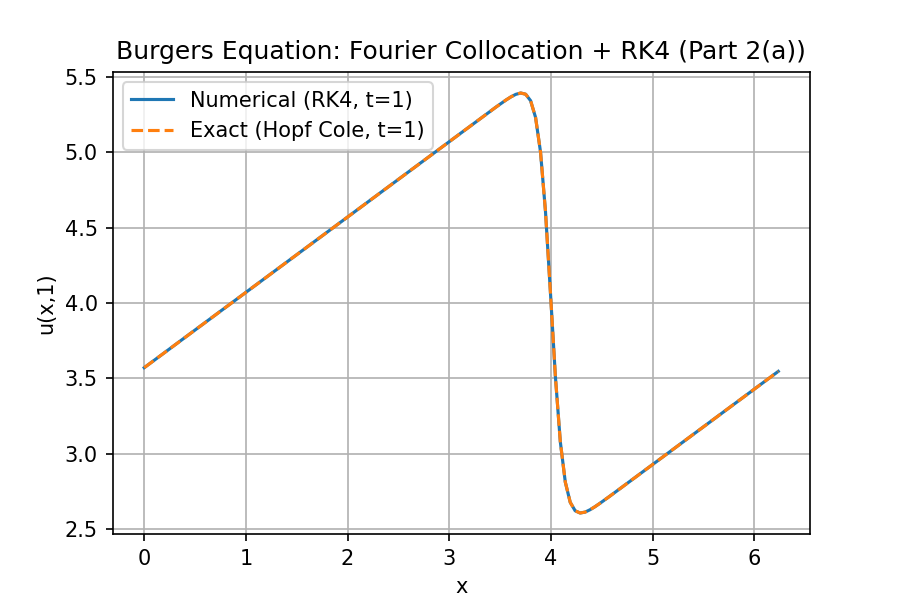
\includegraphics[width=0.9\textwidth]{figure/burgers_solution_part2a.png}
    \caption{Comparison of the numerical solution (RK4) and exact solution (Hopf-Cole) of the periodic Burgers' equation at $t=1.0$. The numerical solution is computed using Fourier Collocation with $N=129$ grid points.}
    \label{fig:burgers_solution_part2a}
\end{figure}

The implementation demonstrates several key features:
\begin{itemize}
    \item High accuracy through spectral differentiation
    \item Stability through adaptive time stepping based on CFL condition
    \item Exact solution validation using the Hopf-Cole transform
    \item Efficient computation using FFT for spatial derivatives
\end{itemize}

\subsection*{(b)}
To investigate the stability of the numerical scheme, we perform a CFL stability analysis using a simple sine wave initial condition. The following code implements the CFL experiment:

\begin{lstlisting}
import numpy as np
import matplotlib.pyplot as plt
import os

def F(u, k, ik, k2, nu):
    u_hat = np.fft.fft(u)
    du_dx = np.fft.ifft(ik * u_hat).real
    d2u_dx2 = np.fft.ifft(-k2 * u_hat).real
    return -u * du_dx + nu * d2u_dx2

def is_stable(u):
    return np.isfinite(u).all()

def try_cfl(N, cfl, c=4.0, nu=0.1, T=np.pi/4, max_steps=10000):
    L = 2 * np.pi
    x = np.linspace(0, L, N, endpoint=False)
    dx = L / N
    u = np.sin(x)  # Simple sine wave initial condition
    k = np.fft.fftfreq(N, d=dx) * 2 * np.pi
    ik = 1j * k
    k2 = k**2
    t = 0.0
    steps = 0
    try:
        while t < T and steps < max_steps:
            dt = cfl / (np.max(np.abs(u)) / dx + nu / dx**2)
            if t + dt > T:
                dt = T - t
            u1 = u + dt/2 * F(u, k, ik, k2, nu)
            u2 = u + dt/2 * F(u1, k, ik, k2, nu)
            u3 = u + dt * F(u2, k, ik, k2, nu)
            u = (1/3) * (-u + u1 + 2*u2 + u3 + dt/2 * F(u3, k, ik, k2, nu))
            t += dt
            steps += 1
            if not is_stable(u):
                return False
        if steps >= max_steps:
            return False
    except Exception as e:
        return False
    return True

N_list = [16, 32, 48, 64, 96, 128, 192, 256]
cfl_values = np.arange(0.05, 2.05, 0.05)
results = {}

for N in N_list:
    max_cfl = 0
    for cfl in cfl_values:
        if try_cfl(N, cfl):
            max_cfl = cfl
        else:
            break
    results[N] = max_cfl
    print(f'N={N}, max stable CFL={max_cfl}')

os.makedirs('figure', exist_ok=True)
plt.figure()
plt.plot(list(results.keys()), list(results.values()), marker='o')
plt.xlabel('N (number of grid points)')
plt.ylabel('Max stable CFL')
plt.title('Max stable CFL vs N for Burgers equation (T=np.pi/4)')
plt.grid(True)
plt.savefig('figure/burgers_cfl_stability.png', dpi=150)
plt.close()
\end{lstlisting}

\subsection*{CFL Stability Results}
Figure~\ref{fig:burgers_cfl_stability} shows the maximum stable CFL number for different grid resolutions.

\begin{figure}[htbp]
    \centering
    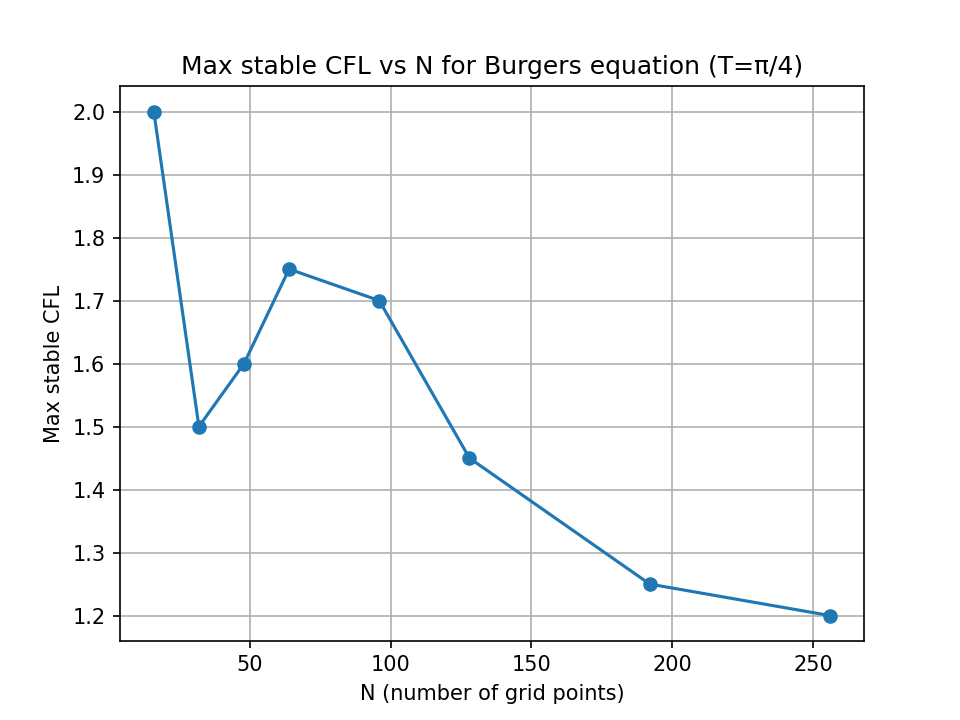
\includegraphics[width=0.9\textwidth]{figure/burgers_cfl_stability.png}
    \caption{Maximum stable CFL number versus grid resolution for the Burgers' equation using a sine wave initial condition.}
    \label{fig:burgers_cfl_stability}
\end{figure}

As shown in Figure~\ref{fig:burgers_cfl_stability}, the maximum stable CFL number decreases as the grid resolution increases. This is consistent with the theoretical expectation that higher resolution requires smaller time steps for stability. The results demonstrate that the numerical scheme remains stable for a wide range of CFL numbers, particularly at lower resolutions.

\end{document} 